\documentclass[letterpaper]{article}
\usepackage[affil-it]{authblk}

\usepackage{amsmath}
\usepackage{amsthm}

%%%%%%%%%%%%%%%%%%%%%%%%%%%%%%%%%%%%%%%%
                                       %
% change this line for portable code:  %
\newcommand*{\commonDir}{./common/}    %
\input{\commonDir preambleCommon}      %
                                       %
%%%%%%%%%%%%%%%%%%%%%%%%%%%%%%%%%%%%%%%%
\usepackage[numbers,sort&compress]{natbib}
\bibliographystyle{unsrtnat}

\graphicspath{{./epistasisEnvFBA/figures/}}

\usepackage{url}
\usepackage{fullpage}
\usepackage{setspace}

\captionsetup[ruled]{labelsep=period}
\makeatletter
\@addtoreset{algorithm}{section}% algorithm counter resets every section
\makeatother
\renewcommand{\thealgorithm}{\thesection.\arabic{algorithm}}% Algorithm # is <section>.<algorithm>

\title{Dynamic Epistasis under Varying Environmental Perturbations}



\date{\today}

%%%%%%%%%%%%%%%%%%
\begin{document}%%
%%%%%%%%%%%%%%%%%%

\newcounter{LinBrandonCoAuthor}
\author[1]{Brandon Barker\footnote{contributed equally}%
\protect\setcounter{LinBrandonCoAuthor}{\value{footnote}}%
}
%  \thanks{contributed equally}
%\addtocounter{footnote}{-1}
\newcommand\LinBrandonCoAuthorMark{\footnotemark[\value{LinBrandonCoAuthor}]}%

\author[2]{Lin Xu\protect\LinBrandonCoAuthorMark}

%\author[2,3]{Brandon Barker}
%\setcounter{footnote}{\value{LinBrandonCoAuthor}}

\author[3,4]{Zhenglong Gu%
  \thanks{Electronic address: \texttt{zg27@cornell.edu}; Corresponding author}}

\affil[1]{Center for Advanced Computing,
    Cornell University, Ithaca, NY, USA.}
\affil[2]{Division of Hematology/Oncology, Department of Pediatrics,
    University of Texas Southwestern Medical Center, Dallas, TX, USA}
\affil[3]{Division of Nutritional Sciences, Cornell University,
  Ithaca, NY, USA.}
\affil[4]{Tri-Institutional Training Program in Computational
  Biology and Medicine, New York, NY, USA.}


\newboolean{thesisStyle}
\setboolean{thesisStyle}{true} 

\maketitle

%%%%%%%%%%%%%%%%%%%%%%%%%%%%%%%%%%%%%%%%
                                       %
\input{\commonDir documentHeadCommon}  %
                                       %
%%%%%%%%%%%%%%%%%%%%%%%%%%%%%%%%%%%%%%%%

\begin{abstract}
\epistasisEnviroAbstract
\end{abstract}

% Redefine suppOrApp
\def\suppOrApp{}


%%%%%%%%%%%%%%%%%%%%%%%%%%%%%%%%%%%%%%%%
%                                      %
\input{\commonDir epistasisEnviroFBA}  %
%                                      %
%%%%%%%%%%%%%%%%%%%%%%%%%%%%%%%%%%%%%%%%

\section{Supporting Information}

\begin{figure}[!htb]
\centering
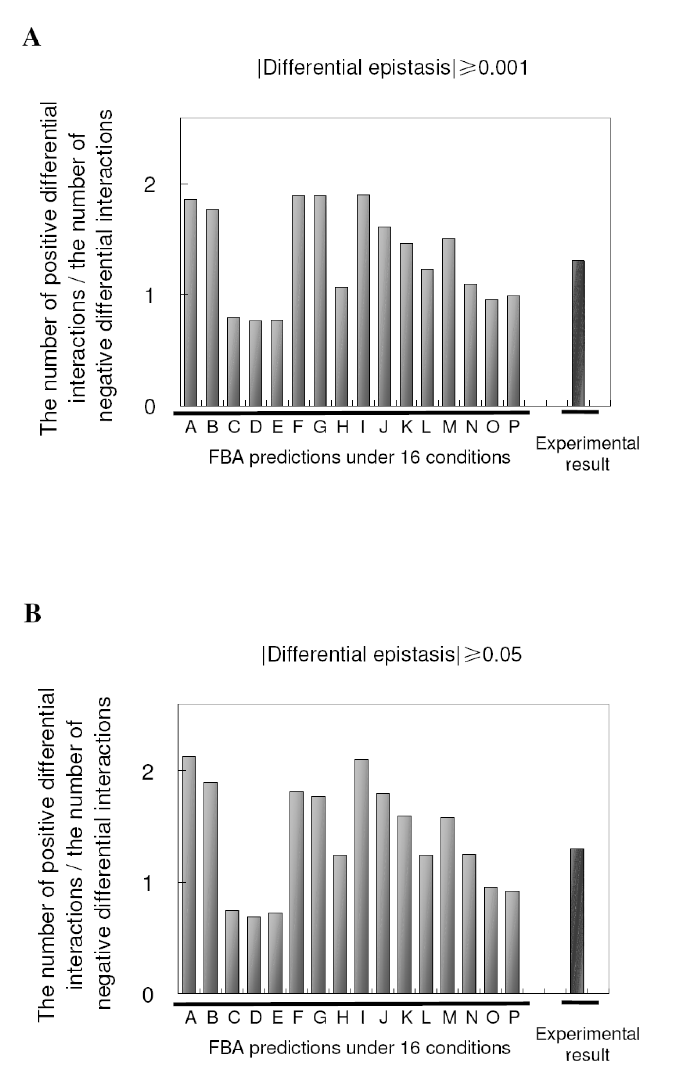
\includegraphics[height=0.8\textheight]{envFigure_S1}
\caption{\eeFBAfigSOneCap}
\label{fig:eefS1}
\end{figure}

\begin{figure}[!htb]
\centering
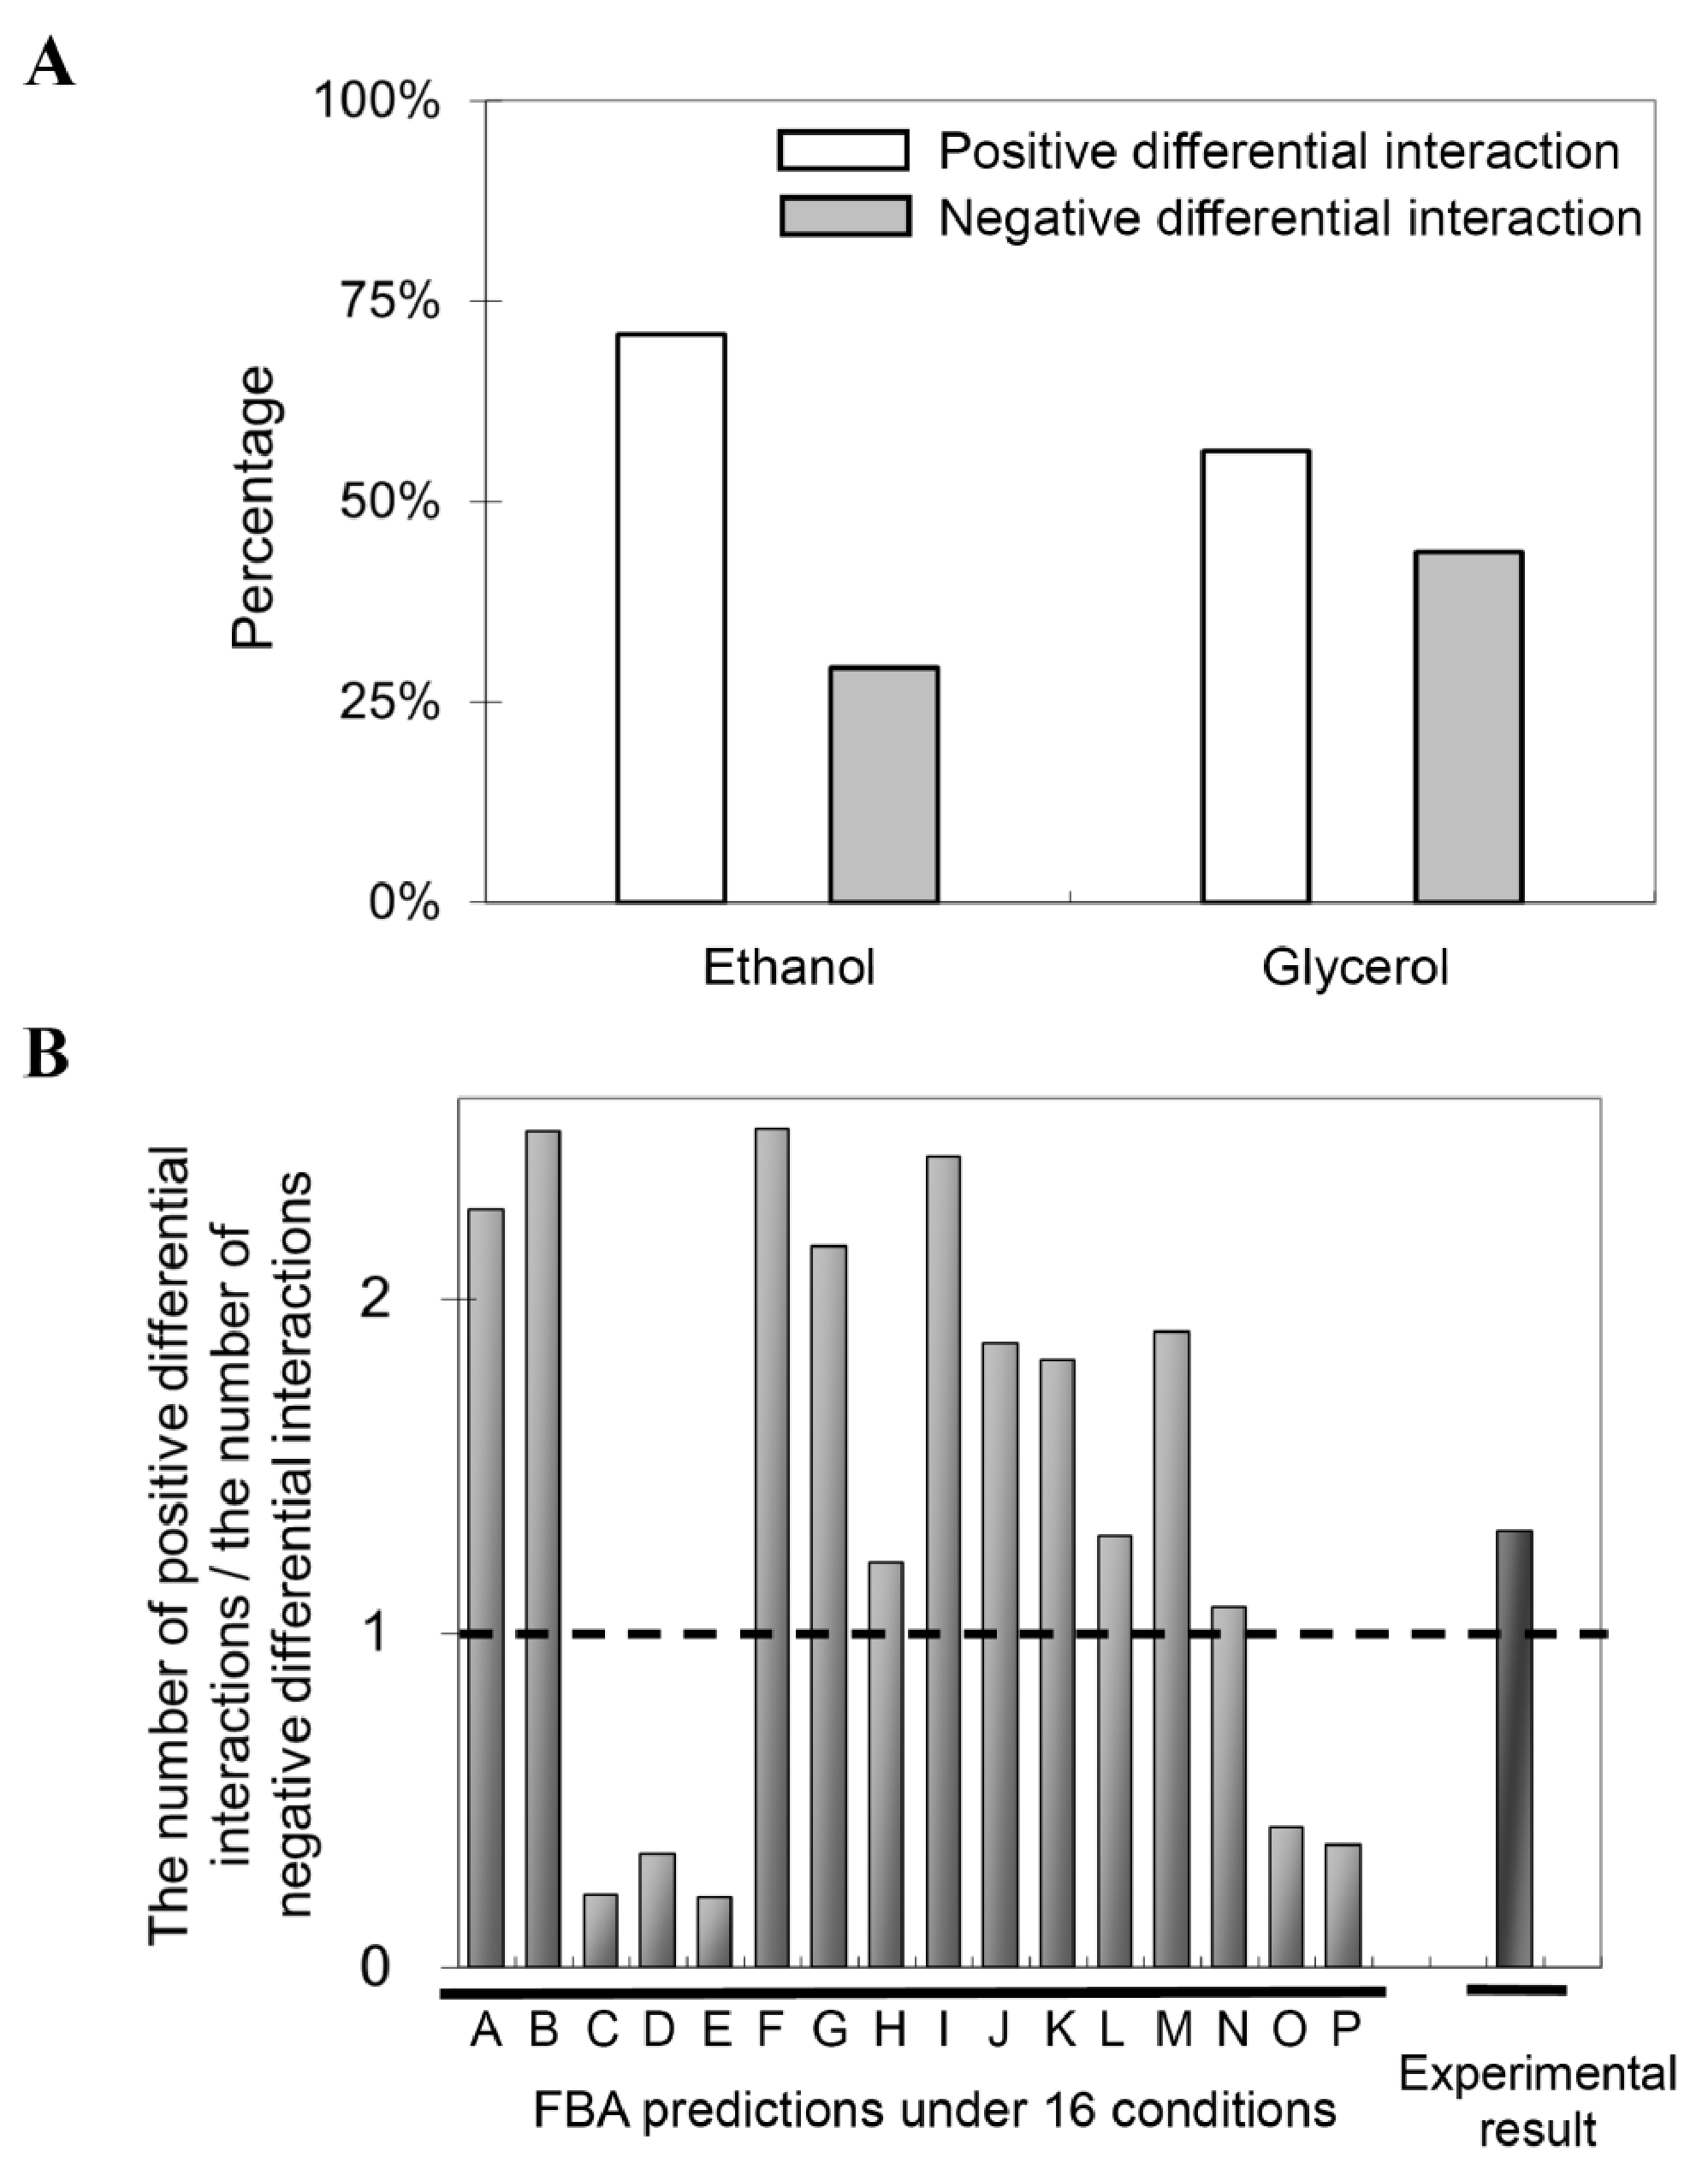
\includegraphics[width=0.8\textwidth]{envFigure_S2}
\caption{\eeFBAfigSTwoCap}
\label{fig:eefS2}
\end{figure}

\begin{figure}[!htb]
\centering
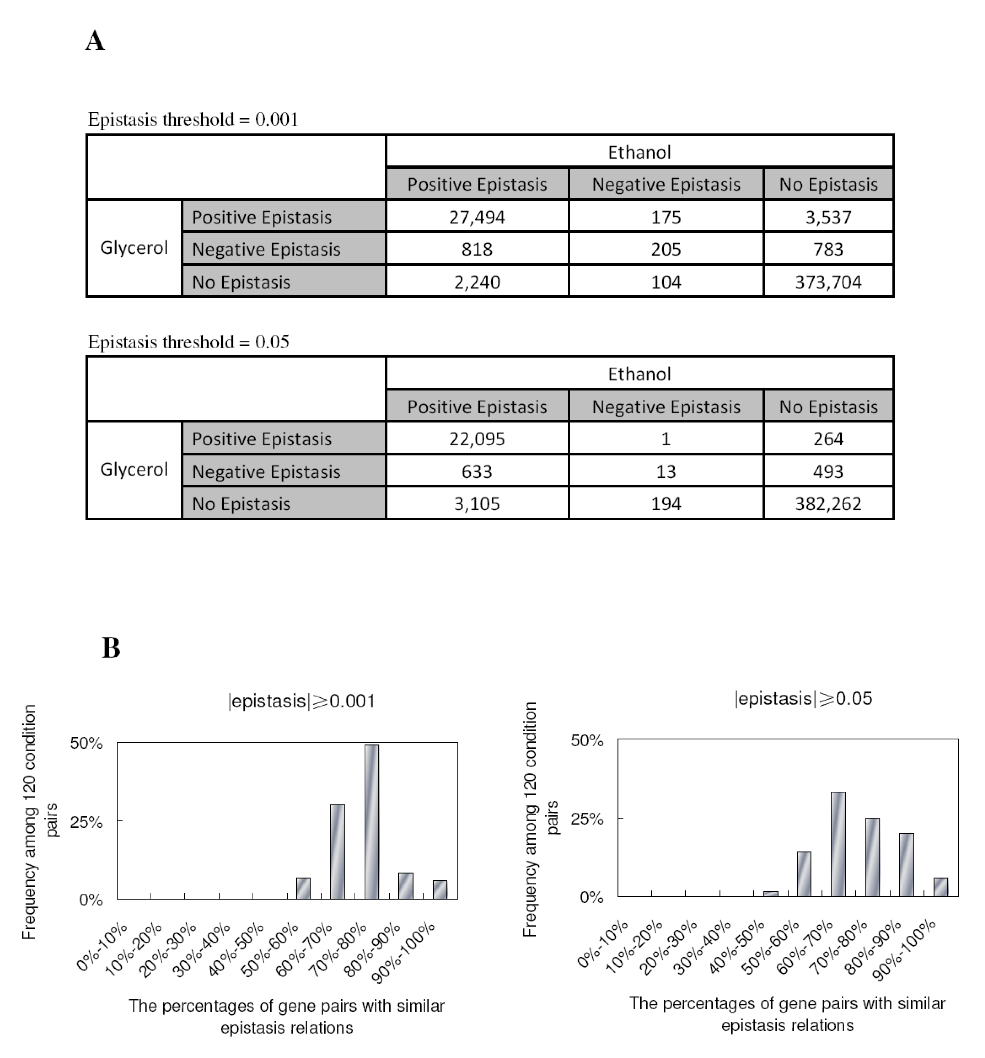
\includegraphics[width=\textwidth]{envFigure_S3}
\caption{\eeFBAfigSThreeCap}
\label{fig:eefS3}
\end{figure}

\begin{figure}[!htb]
\centering
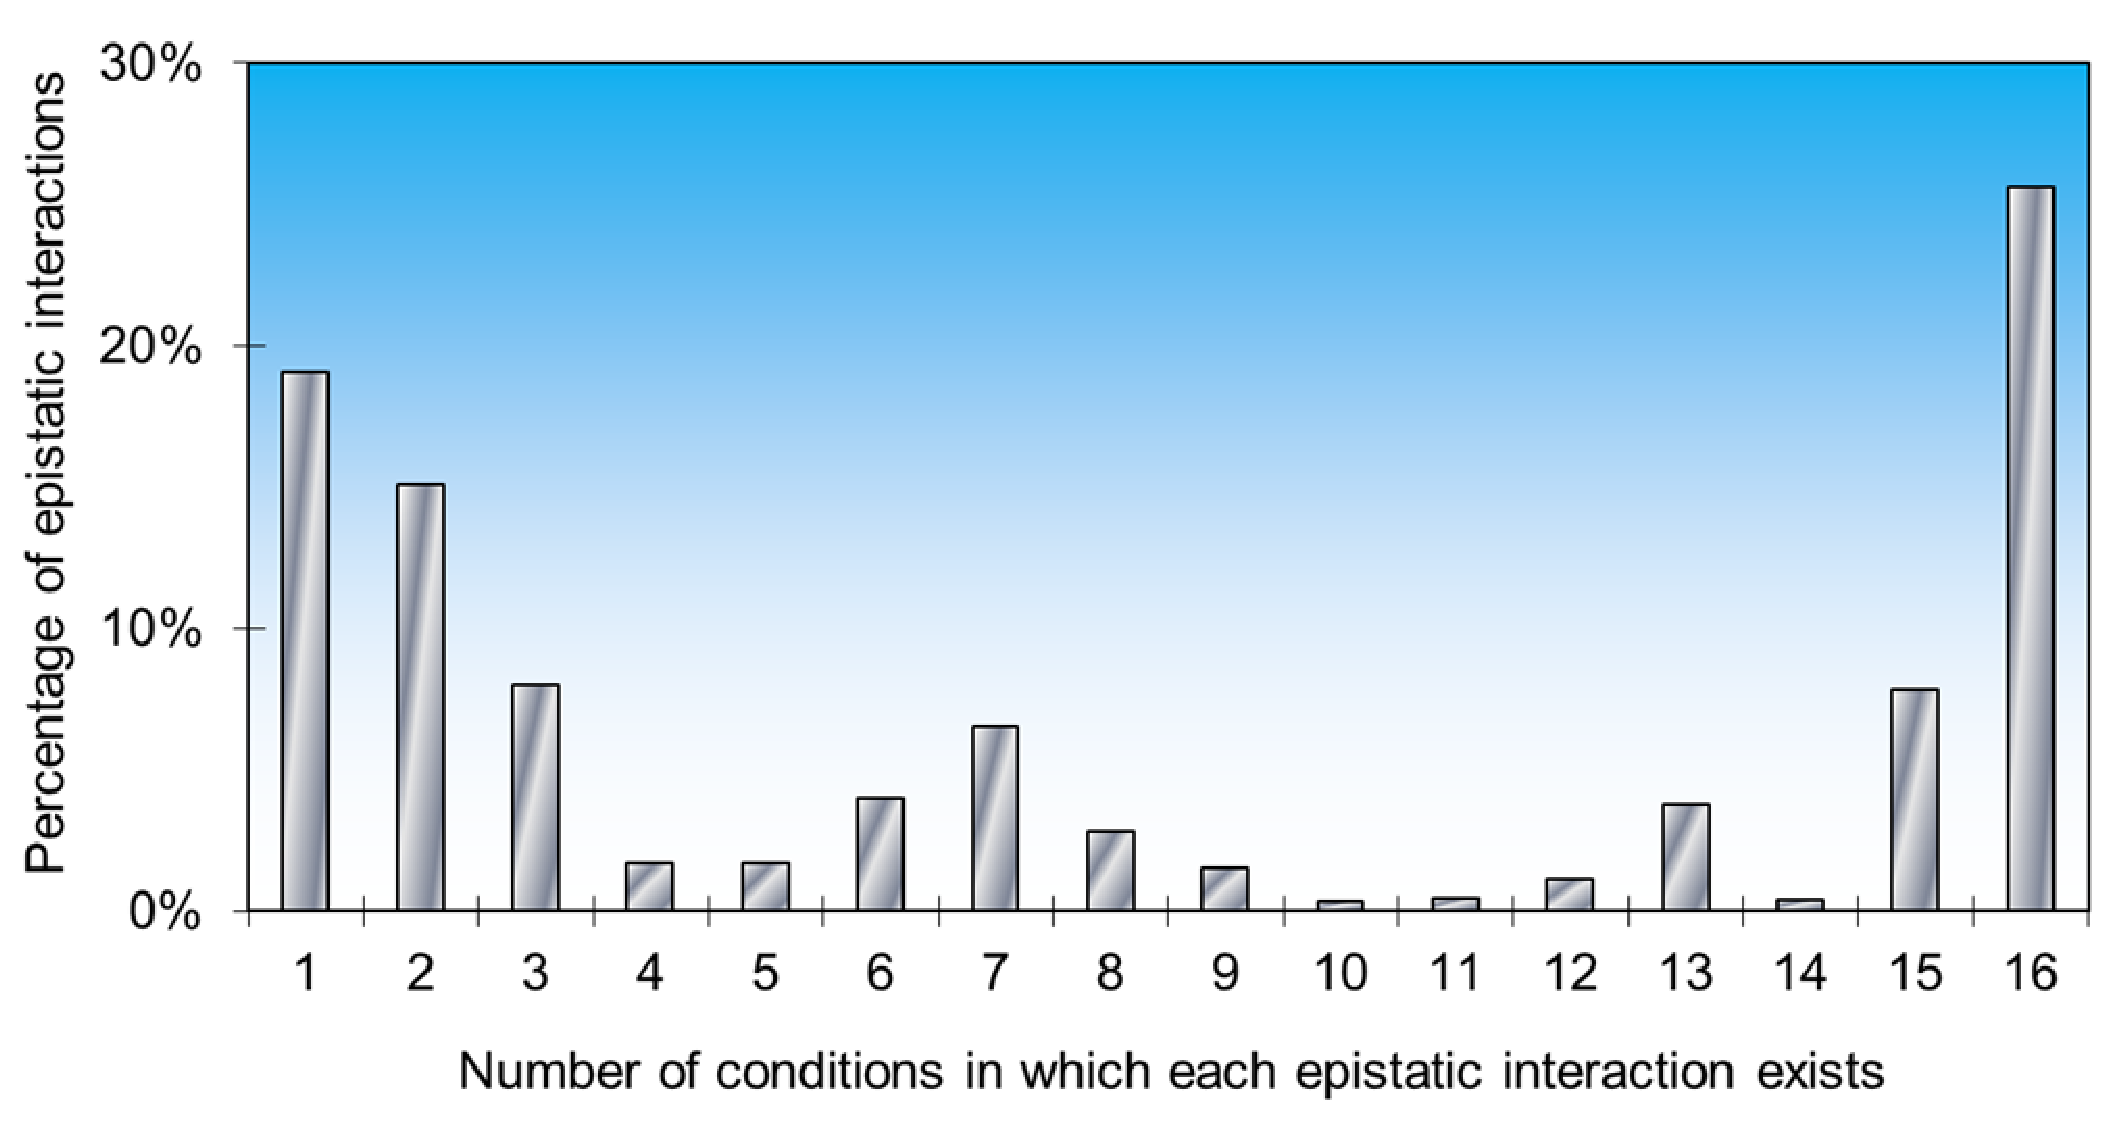
\includegraphics[width=\textwidth]{envFigure_S4}
\caption{\eeFBAfigSFourCap}
\label{fig:eefS4}
\end{figure}

\noindent\textbf{Table S1.} 
\eeFBATabSOneCap

\hspace{1ex}

\noindent\textbf{Table S2.} 
\eeFBATabSTwoCap

\hspace{1ex}

\noindent\textbf{Table S3.} 
\eeFBATabSThreeCap

\hspace{1ex}

\noindent\textbf{Table S4.}
\eeFBATabSFourCap

\hspace{1ex}

\noindent\textbf{Table S5.}
\eeFBATabSFiveCap

\hspace{1ex}

\noindent\textbf{Table S6.}
\eeFBATabSSixCap

\clearpage

\bibliography{library}
\end{document}
